\section{Introduction}

La Terre est constamment bombardée par des rayons cosmiques, majoritairement composés de particules chargées dont des protons et noyaux d'Hélium. Ces particules peuvent atteindre des énergies très importantes ($10^{15}$ à $10^{20}$ eV). Lorsqu'elles pénètrent l'atmosphère, les particules primaires du rayonnement cosmique produisent des particules secondaires instables ayant un temps de vie très court. Ces particules secondaires sont très énergétiques et ultra-relativistes. Elles vont, à leur tour, de nouveau interagir avec des molécules de l'atmosphère ou se désintégrer en particule plus légère. Les cascades de particules qui en résultent sont appelées \textit{gerbes atmosphériques}. Une composante majeure de ces gerbes sont les muons. Ils se propagent jusqu'à la surface de la Terre et sont capables de voyager quelques kilomètres sous la surface avant d'interagir.

Dans ce cours, nous utiliserons ces particules atmosphériques pour démontrer et étudier les méthodes technologiques, expérimentales et analytiques fréquemment utilisées pour détecter les particules subatomiques. Cela se fera à l'aide de quatre dispositifs différents, qui partagent néanmoins des caractéristiques et des techniques communes.

\begin{figure}[hb]
    \center{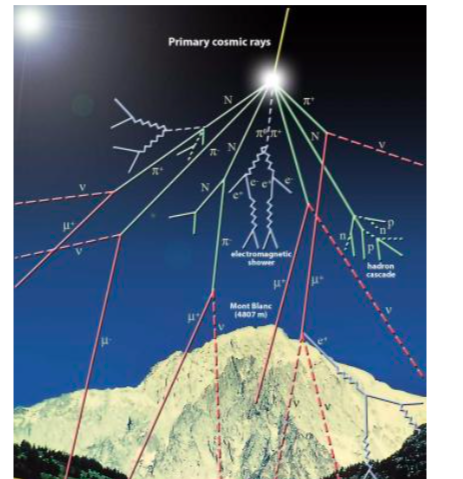
\includegraphics[width=0.56\textwidth]
    {figures/cosmic_rays.png}}
    \caption{\label{fig:CR} Représentation schématique de rayons cosmiques interagissant dans la haute atmosphère.}
\end{figure}

